% Fig. 1 v3 (old Fig. 1 teaser + old Fig. 2 three-axis comparison), full width in the title block, WITH the top scene strip.
% Source: paper/figures/fig01_teaser/v3/fig01_v3.pdf (+ fig01_v3.json: per-panel file, sha256, crop, run/episode/chunk, edits).
% Script: paper/tools/plotting/cvpr_v3_fig1_compose.py. Variant without the top strip: figure_v3_notop.tex.
\begin{minipage}{\textwidth}
\centering
\captionsetup{type=figure,hypcap=false}
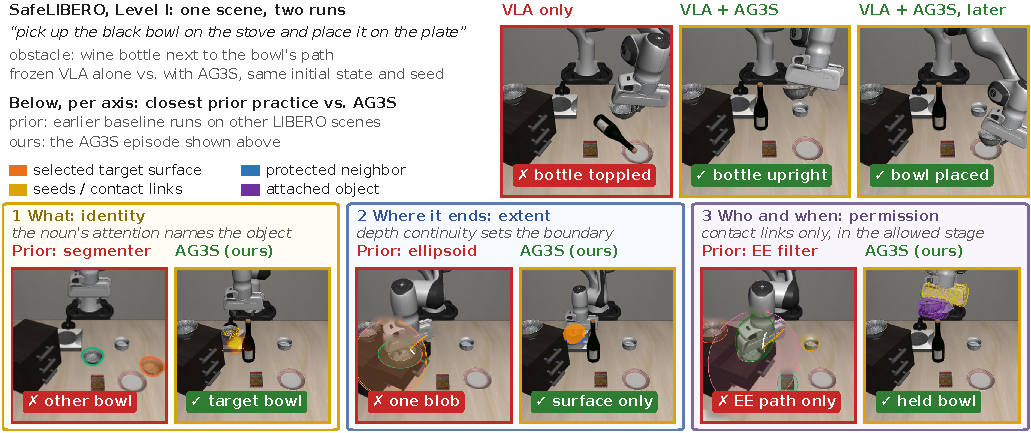
\includegraphics[width=\textwidth]{../figures/fig01_teaser/v3/fig01_v3.pdf}
\caption{\textbf{One frozen VLA decides what may be touched, where that surface ends, and by which link, when.}
\emph{Top:} in a SafeLIBERO Level~I scene with a wine bottle next to the bowl's path, the frozen $\pi_{0.5}$ completes ``pick up the black bowl on the stove and place it on the plate'' by knocking the bottle over (left); with \sys, from the same initial state and seed, the bottle is still upright at the same step (middle) and the bowl is placed (right).
\emph{Bottom, each axis against the closest prior practice.}
\emph{Identity:} Grounded-SAM-2~\cite{liu2024groundingdino,ravi2024sam2} prompted with the instruction fills a second bowl (orange; green outline: the instructed bowl), whereas the policy's own noun attention, lifted to the observed points, seeds the bowl it acts on (gold).
\emph{Extent:} ellipsoids fitted to detected objects (AEGIS~\cite{hu2026vlsa}) enclose the cabinet together with the bowl inside it; depth continuity bounds the bowl's observed surface (orange) and keeps the adjacent geometry protected (blue).
\emph{Permission:} a filter on the end-effector path against object ellipsoids (KNOWS$^\ast$~\cite{park2026knows}) has no notion of a carried object; \sys\ frees the target surface only for the contact links (gold) and, once grasped, protects the bowl as attached geometry (purple).
Prior panels are outputs of the baseline implementations on LIBERO scenes without obstacles, from earlier runs and not the episode above; their small name tags are removed and the segmenter mask is recolored to our code. The top row and our panels are recorded frames of one SafeLIBERO episode; the two runs share initial state and seed.}
\label{fig:teaser}
\end{minipage}
